\begin{figure}
    \centering
    \begin{tabular}{c c c c}
         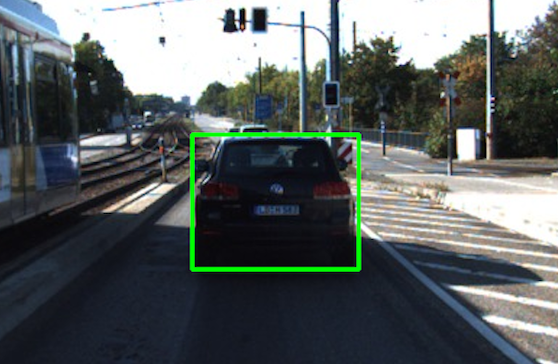
\includegraphics[height=0.135\textwidth]{figures/method/ambiguous/ex4/rgb.png}
        &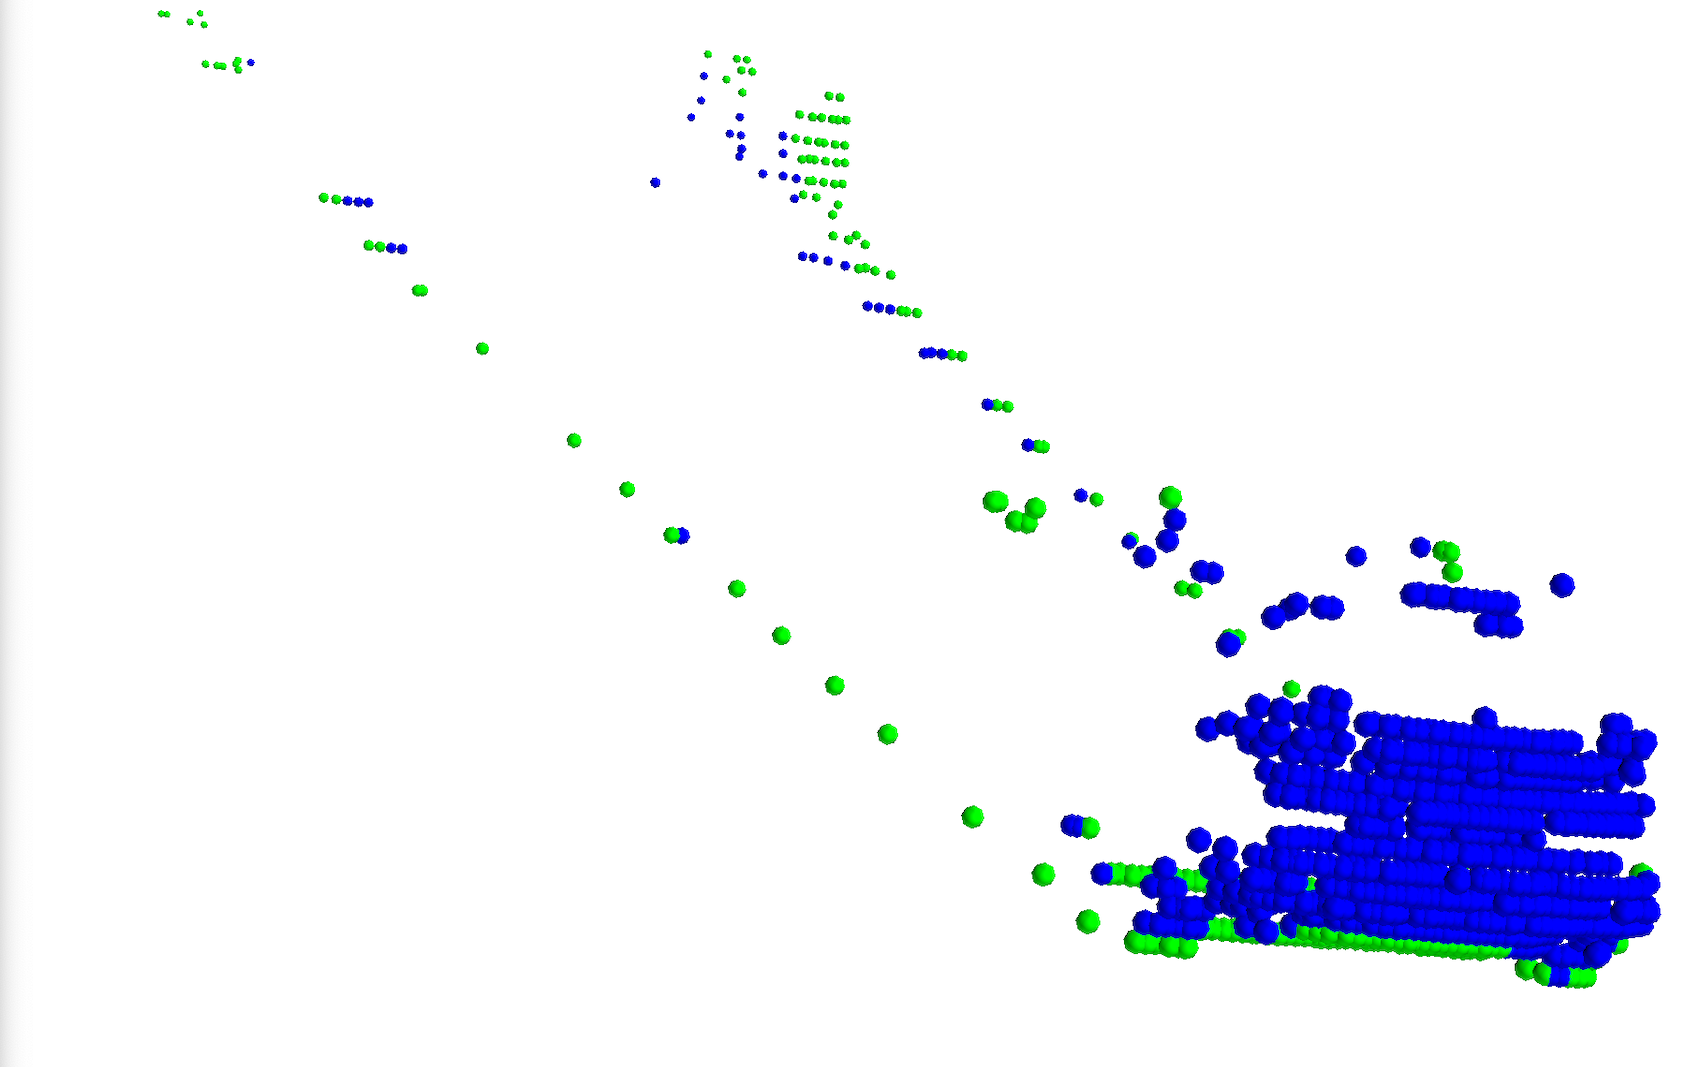
\includegraphics[height=0.135\textwidth]{figures/method/ambiguous/ex4/pcd.png} &
         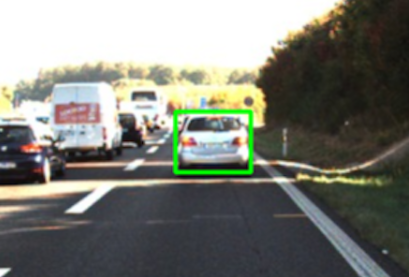
\includegraphics[height=0.135\textwidth]{figures/method/ambiguous/ex6/rgb.png}
        &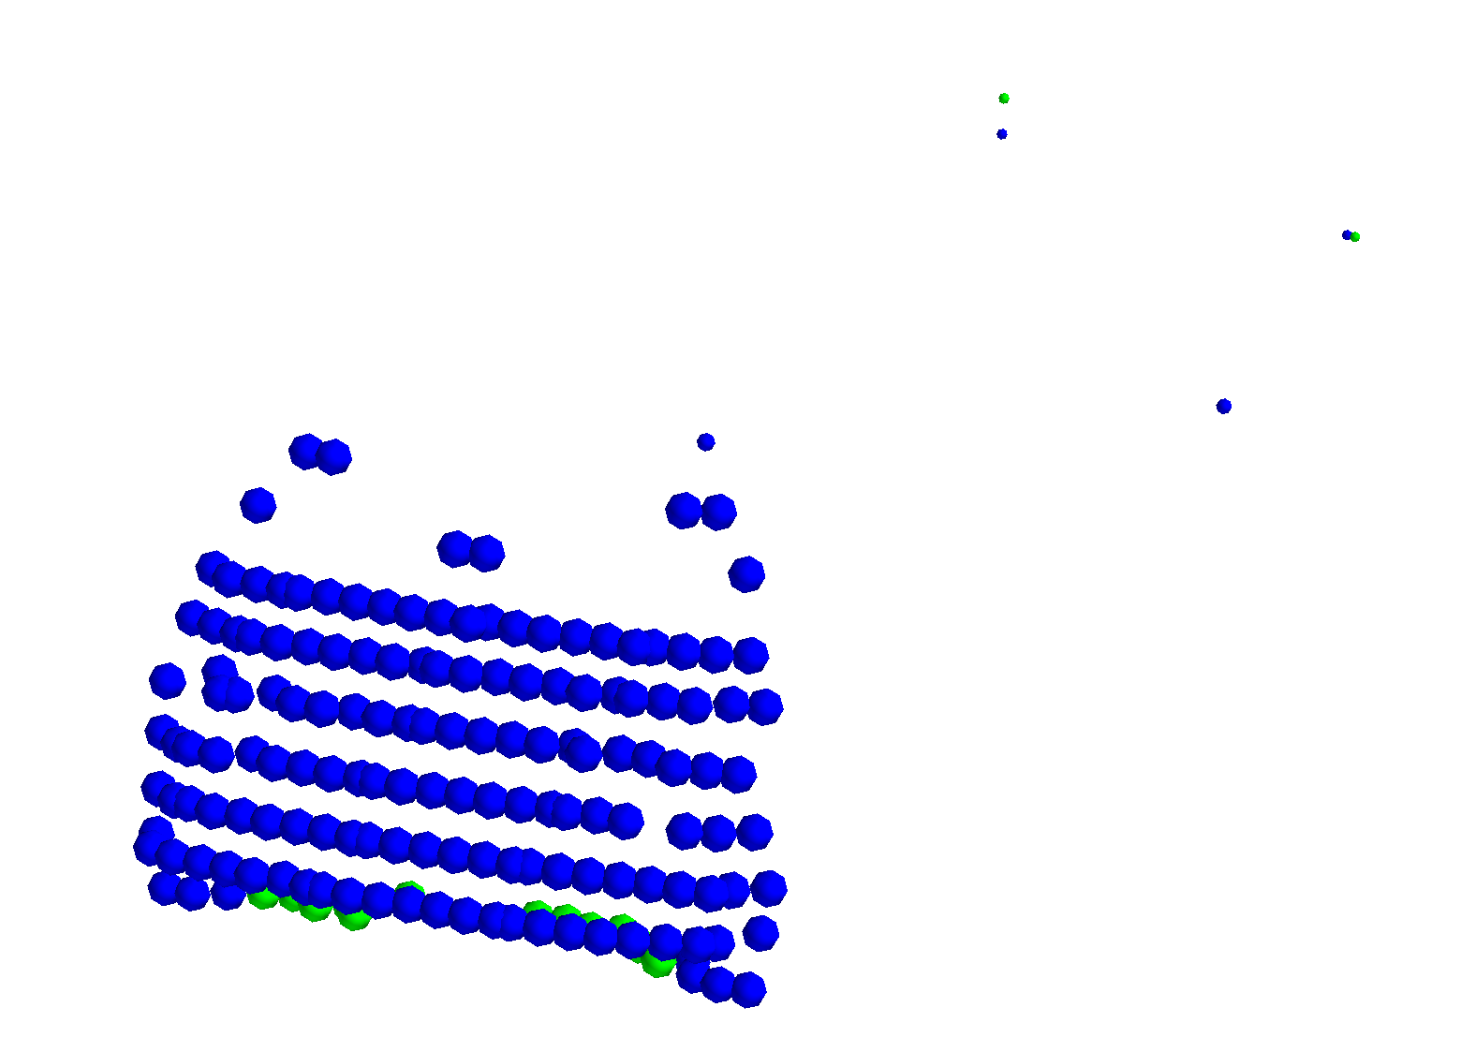
\includegraphics[height=0.135\textwidth]{figures/method/ambiguous/ex6/pcd.png}
    \end{tabular}
    \caption{In some cases the LiDAR point cloud only captures a single surface of the vehicle. This is problematic as fitting such point clouds is ambiguous, particularly for the rotation component.}\label{fig:ambiguous}
\end{figure}